% p19-f-circ-unsmash-completes-the-following-diagram.tex
%
% Source:   Carl A. Gunter and Dana S. Scott, "Semantic Domains".
%           ScottDomains/papers/Gunter Scott 1990.pdf
% Physical page: 19          Printed page: 18
% Section:  4.3 Smash products.
% Unnamed in the paper (no figure number). Introduced by:
%   "If f : D x E -> F is bistrict and continuous, then g = f o unsmash is the
%    unique strict, continuous function which completes the following diagram:"
%
% Content: a commutative triangle. Solid arrows are maps the text has already
% named; the dashed arrow is the unique map whose existence the sentence
% asserts. Vertices 3, arrows 3 (2 solid, 1 dashed).
%
% Geometry measured from a 300 dpi render of the region and divided by
% 118.11 px/cm.
%
\documentclass[border=6pt]{standalone}
\usepackage{tikz}
\begin{document}
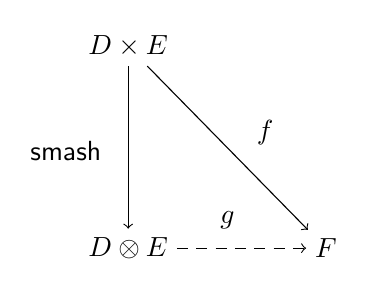
\begin{tikzpicture}[
  x=1cm, y=1cm,
  every node/.style={inner sep=1pt},
  open/.style={circle, draw, fill=white, minimum size=4pt, inner sep=0pt},
  solid/.style={circle, draw, fill=black, minimum size=5pt, inner sep=0pt},
  edge/.style={draw, line width=0.4pt},
  % added for the commutative diagrams: object nodes, and the paper's two
  % arrow kinds -- solid for a named map, dashed for the unique completing map
  obj/.style={inner sep=3pt},
  arrow/.style={draw, line width=0.4pt, ->},
  darrow/.style={draw, line width=0.4pt, ->, dash pattern=on 4pt off 3pt}]

  % vertices
  \node[obj] (dxe) at (0.00,2.56) {$D \times E$};
  \node[obj] (dte) at (0.00,0.00) {$D \otimes E$};
  \node[obj] (f)   at (2.51,0.00) {$F$};

  % arrows
  \draw[arrow]  (dxe) -- (dte);
  \draw[arrow]  (dxe) -- (f);
  \draw[darrow] (dte) -- (f);

  % labels printed inside the picture
  \node[anchor=east] at (-0.30,1.24) {\textsf{smash}};
  \node at (1.74,1.47) {$f$};
  \node at (1.26,0.36) {$g$};
\end{tikzpicture}
\end{document}
